%\title{Presentation Template}
\documentclass[10pt]{beamer}

\usetheme[progressbar=frametitle]{metropolis}
\usepackage{appendixnumberbeamer}

\usepackage[compatibility=false]{caption}
\usepackage{subcaption}
\usepackage{csquotes}
\usepackage{booktabs}
\usepackage{hyperref}
\usepackage[scale=2]{ccicons}
\usepackage{fontawesome}
\usepackage{tikz}
\usepackage{bm}
\usepackage{adjustbox}

\usepackage{footnpag} %reset footnotes at every page

\makeatother
\renewcommand{\thefootnote}{\ifcase\value{footnote}\or*\or
**\or***\or****\fi}
\makeatletter

\makeatletter\newcommand\HUGE{\@setfontsize\Huge{28}{34}}\makeatother

\graphicspath{{./img/}}

\usepackage{pgfplots}
\usepgfplotslibrary{dateplot}

\usepackage{xspace}
\newcommand{\themename}{\textbf{\textsc{metropolis}}\xspace}

\newfontfamily\sansforgetica{SansForgetica-Regular.otf}

\title{TITLE}
\subtitle{EVENT}
\date{DATE}
\author{Matthew Andres Moreno \newline {\faTwitter} @MorenoMatthewA \newline}
\titlegraphic{\vspace{32ex}\hfill\includegraphics[height=2.5cm]{img/BEACON-logo}}
\newcommand{\projecturl}{https://osf.io/TODO}

\begin{document}

\maketitle

% \begin{frame}{Table of contents}
%   \setbeamertemplate{section in toc}[sections numbered]
%   \tableofcontents[hideallsubsections]
% \end{frame}

\section{Section}

\begin{frame}{Slide Title}
\begin{columns}
\begin{column}{0.6\textwidth}
\begin{itemize}
\item data management
\item foo
\end{itemize}
\end{column}
\begin{column}{0.4\textwidth}
\begin{center}
words
\end{center}
\end{column}
\end{columns}
\end{frame}

\begin{frame}{Animation}

\begin{figure}

\foreach \n in {1,...,7}{%
\includegraphics<\n>[width=\textwidth]{ant-bridge/frame-\n}%
}%

\caption{
\textit{Eciton} army ants use living bridges to create a foraging shortcut.
Bridge placement, determined by decentralized ant-to-ant interactions, maximizes foraging rate.
Graphics from \cite{reid2015army}.
}

\end{figure}


\end{frame}


\appendix

\appendix

\begin{frame}{For More Information}

\vspace{1ex}

\begin{adjustbox}{width=\textwidth,center}%
{\HUGE\url{\projecturl}}%
\end{adjustbox}

\vspace{3ex}

\begin{itemize}
\item live in-browser demo
\item source code
\item data
\item figures and graphics
\item how-to-replicate tutorial
\item publication
\item slides
\end{itemize}

\end{frame}

\begin{frame}{People}

\begin{columns}
\begin{column}{0.25\textwidth}
  \centering
  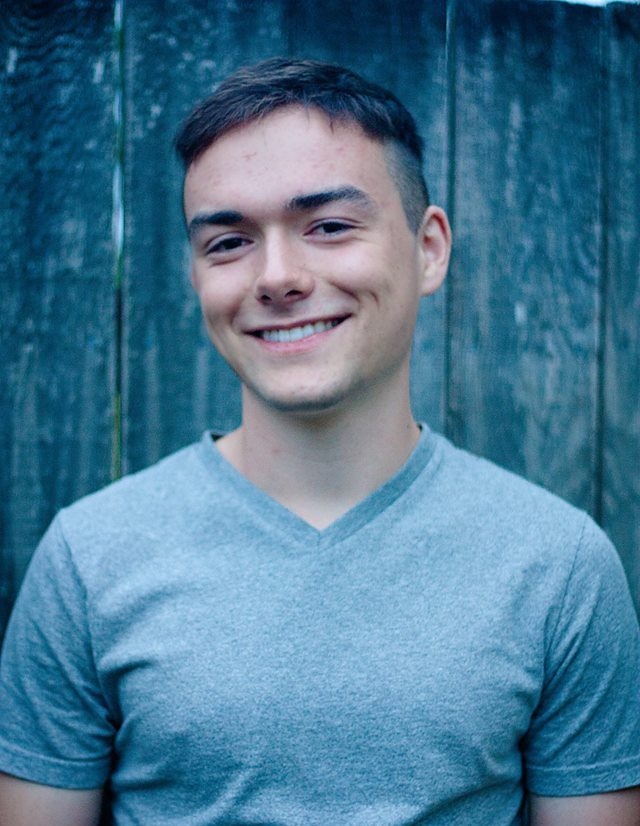
\includegraphics[width=0.7\textwidth]{moreno}
\end{column}
\begin{column}{0.75\textwidth}
  \textbf{Matthew Andres Moreno}

  \href{https://twitter.com/MorenoMatthewA}{{\faTwitter} @MorenoMatthewA}

  \href{https://mmore500.github.io}{{\faGlobe} \texttt{https://mmore500.github.io}}

  \href{mailto: mmore500@msu.edu}{{\faEnvelope} \texttt{mmore500@msu.edu}}

\end{column}
\end{columns}

\vspace{1ex}

\begin{columns}
\begin{column}{0.25\textwidth}
  \centering
  \includegraphics[width=0.7\textwidth]{ofria}
\end{column}

\begin{column}{0.75\textwidth}
  \textbf{Charles Ofria}

  \href{https://twitter.com/CharlesOfria}{{\faTwitter} @CharlesOfria}

  \href{https://ofria.com}{{\faGlobe} \texttt{https://ofria.com}}

  \href{mailto: ofria@msu.edu}{{\faEnvelope} \texttt{ofria@msu.edu}}

\end{column}
\end{columns}
\vfill
\begin{columns}
\begin{column}{0.5\textwidth}
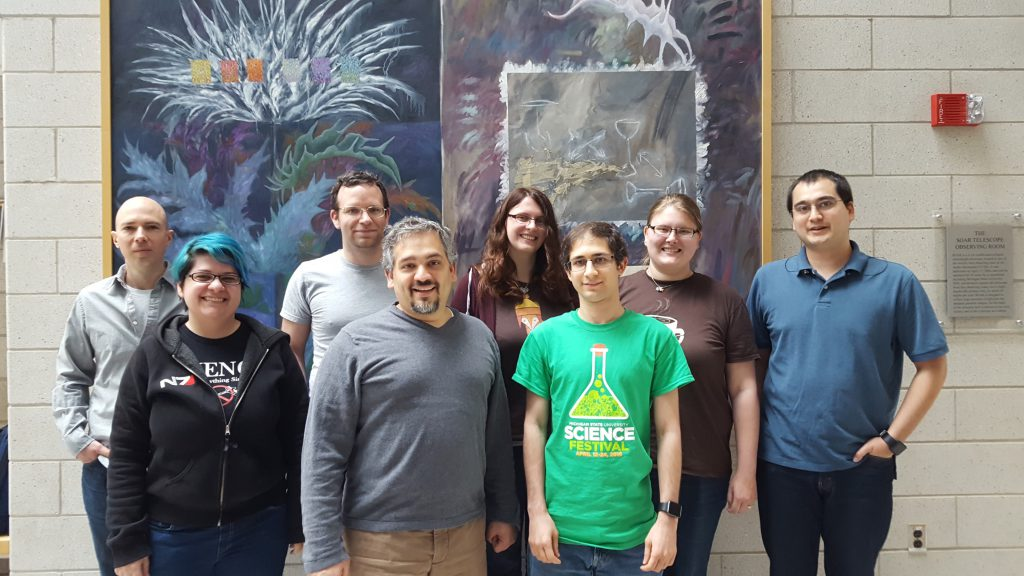
\includegraphics[width=\textwidth, trim={0 0 0 150}, clip]{group_photo}
\end{column}
\begin{column}{0.5\textwidth}

\includegraphics[width=\textwidth]{devolab-logo}
\end{column}
\end{columns}

\end{frame}

\begin{frame}{Acknowledgements}
\small
\begin{itemize}
\item Empirical Library for scientific software development in C++
\item Open Science Framework via the Center for Open Science
\item computational resources via Michigan State University's Institute for Cyber-Enabled Research
\item This material is based upon work supported by the National Science Foundation Graduate Research Fellowship under Grant No. DGE-1424871.\footnote[1]{\label{foot:disclaimer} \tiny Any opinions, findings, and conclusions or recommendations expressed in this material are those of the author(s) and do not necessarily reflect the views of the National Science Foundation.}
\item This research was supported in part by NSF grants DEB-1655715 and DBI-0939454.\footnotemark[1]
\end{itemize}

\vfill

\newcommand{\innerspacer}{0.07\textwidth}
\newcommand{\content}{0.24\textwidth}
\newcommand{\outerspacer}{0.07\textwidth}

\begin{center}
 \begin{columns}
	\begin{column}{\outerspacer}~\end{column}
	 \begin{column}{\content}
		
\includegraphics[width=\textwidth]{NSF-logo}
 	\end{column}
  \begin{column}{\innerspacer}~\end{column}
	 \begin{column}{\content}
		\includegraphics[width=\textwidth]{BEACON-logo}
 	\end{column}
  \begin{column}{\innerspacer}~\end{column}
 	\begin{column}{\content}
   \includegraphics[width=0.75\textwidth]{MSU-helmet}
 	\end{column}
 	\begin{column}{\outerspacer}~\end{column}
 \end{columns}
\end{center}

\end{frame}


\begin{frame}[standout]
\vspace{17ex}

{\Huge
Questions?%
}
\vspace{15ex}

\begin{adjustbox}{width=0.5\textwidth,center}%
\url{\projecturl}%
\end{adjustbox}

\end{frame}

\begin{frame}[allowframebreaks]{References}

  \bibliography{bibl}
  \setbeamertemplate{bibliography item}{\insertbiblabel}
  %\nocite{*} % Insert publications even if they are not cited in the poster
  \bibliographystyle{apalike}
\end{frame}


\input{tex/backup.tex}

\end{document}
